\section{Experiment 4: the importance of edges}

\subsection{Methodology}

\paragraph{Stimuli}

A 1000-frame corpus of consecutive fire images was used.

\paragraph{Subjects}

15 subjects were recruited using a mailing list operated by University College London. All reported normal or corrected-to-normal vision.

\paragraph{Trial structure}

2AFC Delayed match-to-sample with altered sample.
In each trial, a sample was presented first, followed by two tests. A manipulation was applied to the sample; the tests were unchanged. Subjects indicated which test they thought corresponded to the sample using the left arrow (first sample) and right arrow (second sample) keys. 

Sample length (sL) was one 10 frames (0.2 seconds)
Test length was 15 frames (0.3 seconds)

\paragraph{Factors}

In half the trials, the sample was manipulated using a Sobel edge filter. The test clips were left unchanged.

Each frame was convolved with the 3x3 filter

    0.1250    0.2500    0.1250
         0         0         0
   -0.1250   -0.2500   -0.1250

to give an estimate of the image derivative. All pixels above a certain threshold value in the derivative image were returned as edges. The implementation used was MATLAB's edge() function.


\paragraph{Block structure}

Firstly, we presented 30 training trials with static samples and tests (displayed for 0.2 and 0.3 seconds respectively), half of which used the edge-filtered sample.

Next, we presented 15 training trials with dynamic samples and tests and the same clip lengths, but with samples and tests unaltered.

There were 2 block types; we presented each block 7 times (in random order), giving a total of 14 blocks.
We presented 40 trials per block, giving a total of 560 trials.


\begin{figure}[H]
\centering
\renewcommand{\arraystretch}{1.8}

      \begin{subfigure}[b]{\textwidth}
\begin{tabular}{ >{\bfseries}r | p{8cm}   }
& \textbf{Experiment 4}\\
\hline
  
	Design & 2AFC delayed match-to-sample (sample clip followed by two test clips)\\                   
  Stimuli & 1000-frame corpus \\
  Factors & sample edge-filtered or untouched \newline \\
  Block design & 14 blocks, half edge-filtered \newline
280 trials per condition \newline
560 trials \newline
45 training trials \\
Subjects & 15\\
\end{tabular}
\caption{Design summary.}
   \end{subfigure}

\begin{subfigure}[b]{\textwidth}
\centering
                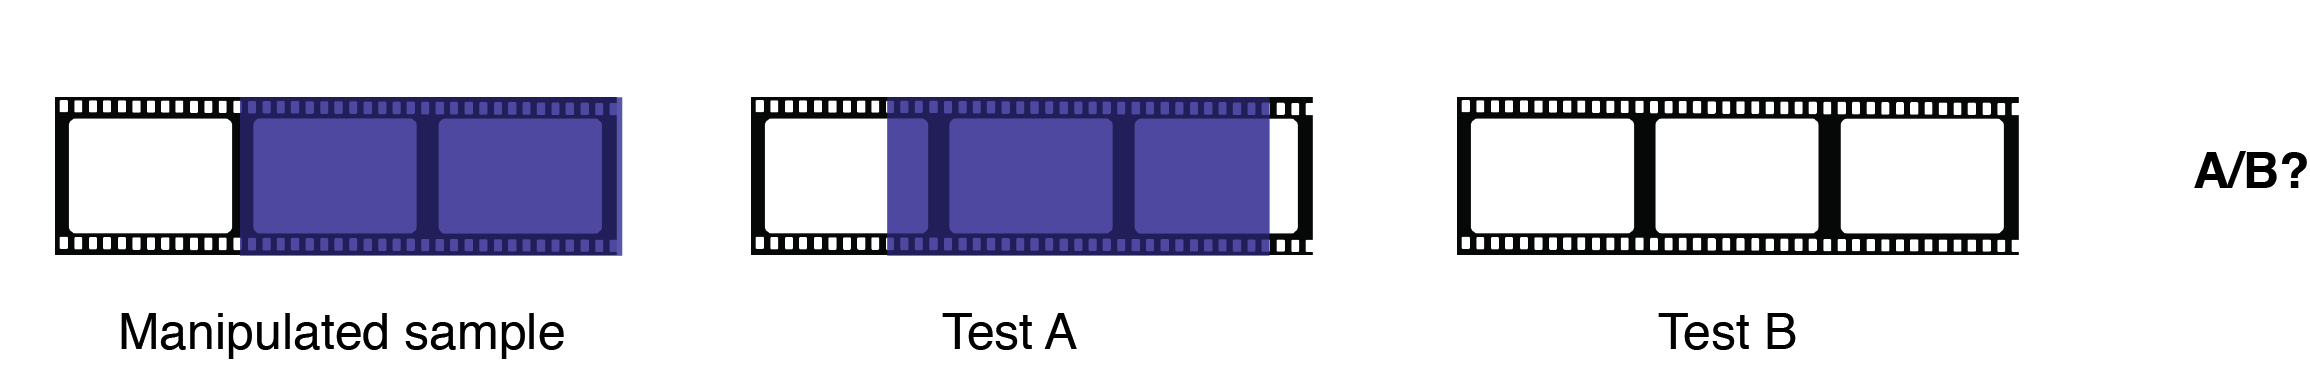
\includegraphics[width=12cm]{img/fire5protocol.png}
                \caption{A short sample was followed by two longer tests, one of which contained the sample.}
         
        \end{subfigure}
\caption{Experiment 4: design summary and trial structure.}
\end{figure}


\subsection{Results}

\paragraph{Edge filtering}

Edge-filtering the sample induced a 4 percentage point drop in accuracy compared to the normal condition:

\begin{center}
\begin{tabular}{ r | l   }
\textbf{Sample} & \textbf{Mean accuracy}\\
\hline
Normal &  0.782\\
Edge-filtered&  0.742\\
\end{tabular}
\end{center}


This difference was significant (paired-samples $t$-test, $p$<0.005).

\paragraph{Order}

Presenting the sample as the first test (as opposed to the second test) induced an accuracy drop of 4.5 percentage points:

\begin{center}
\begin{tabular}{ r | l   }
\textbf{Test order} & \textbf{Mean accuracy}\\
\hline
True test first &  0.785\\
Foil test first&  0.740\\
\end{tabular}
\end{center}

However a paired-samples $t$-test did not find this difference significant ($p$=0.22).




\begin{figure}[htb]
\centering
\begin{subfigure}[b]{\textwidth}
\centering
                
\includegraphics[width=5cm]{img/edges.png}\hspace{0.5cm}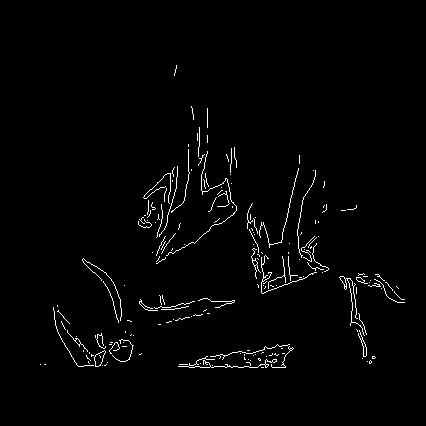
\includegraphics[width=5cm]{img/edges2.png}
                \caption{Two edge-filtered frames.}
         
        \end{subfigure}
\begin{subfigure}[b]{\textwidth}
\centering
                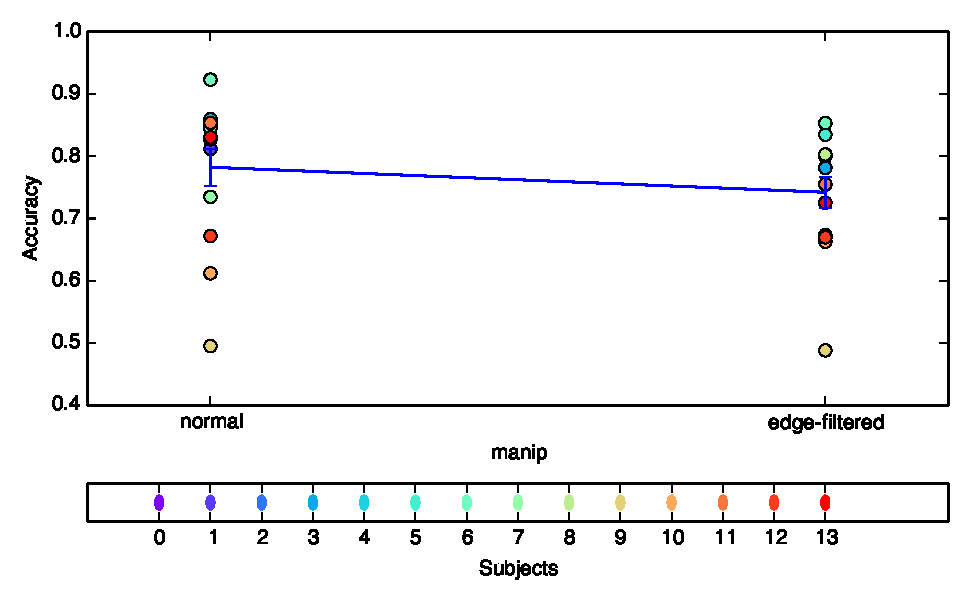
\includegraphics[width=12cm]{img/fig_fire10-edges_correct_manip.pdf}
                \caption{Edge-filtering the samples induced a 4 percentage point accuracy drop.}
      		\label{f:e2:learn}
        \end{subfigure}
\caption{Experiment 4: detecting a sample based on its edges alone.}
\end{figure}

\subsection{Discussion}


Edges are very important in the representation of fire. We are able to match a sample clip from which all of the texture and fine contrast information has been removed, with an unaltered test, with only a small impairment from normal performance. This shows that the visual system is able to extract very useful information from flame edges alone, and employ it effectively for comparison.

This observation allows us to reject the hypothesis that fire matching is done based on the global average luminance signal, which is not preserved under edge filtering.

Edges are very important in the generation of salience maps\cite{alter1998extracting}, which guide attention to features useful for discrimination. The generation of salience percepts is not local, as evidenced by its tendency to highlight features which form global shapes:

\begin{center}
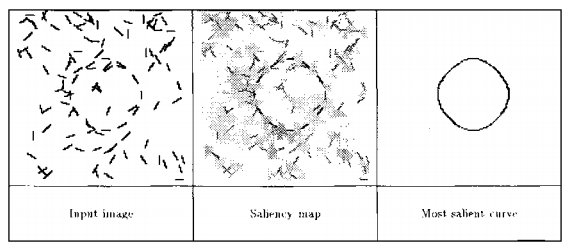
\includegraphics[width=0.7\textwidth]{img/salience}\\
\textit{The circle in the first image is detectable both by your visual system and by the Shashua and Ullman model described by this figure from \cite{alter1998extracting}.}
\end{center}

However, the edges in this experiment were generated purely locally, by convolving each frame with the matrix


\[
M=
  \begin{bmatrix}
    0.125 & 0.25 & 0.125\\
    0 & 0 & 0\\
-0.125 & -0.25 & -0.125\\
  \end{bmatrix}
\]

which is only 3-by-3 and thus very local. Edge detection has often been used as an input to saliency map generators, which are more global; one small object by itself in a large image is very salient, but when surrounded by dozens of similar objects, salience is quickly lost.

Salience-map calculation is related to grouping, but is quite different. We define grouping as the process by which local features are bound together into global features, as, for example, the local edge elements in the image just above are unified into the percept of a circle. It is often assumed that grouping, like salience, can be implemented by a map: a representation composed of local pixel-like elements in which each element is tagged with the identity of the object it belongs to.

There are several problems with this idea:

\begin{itemise}
\item Maps make sense for scalar quantities like luminance and salience, but object identity is not scalar: how do we code \emph{teapot} or \emph{face} in a scalar manner?

\item Maps do not make sense for hierarchical representations: one pixel of a human body can belong to \emph{finger}, \emph{hand}, \emph{arm}, \emph{upper body} and \emph{John}. There is no room in a map to code all of this information.

\item Object segmentation can be a very complex computation and is not always performed unless required. For example, in the following image, we can decide whether two points belong to the same object if asked:

\begin{center}
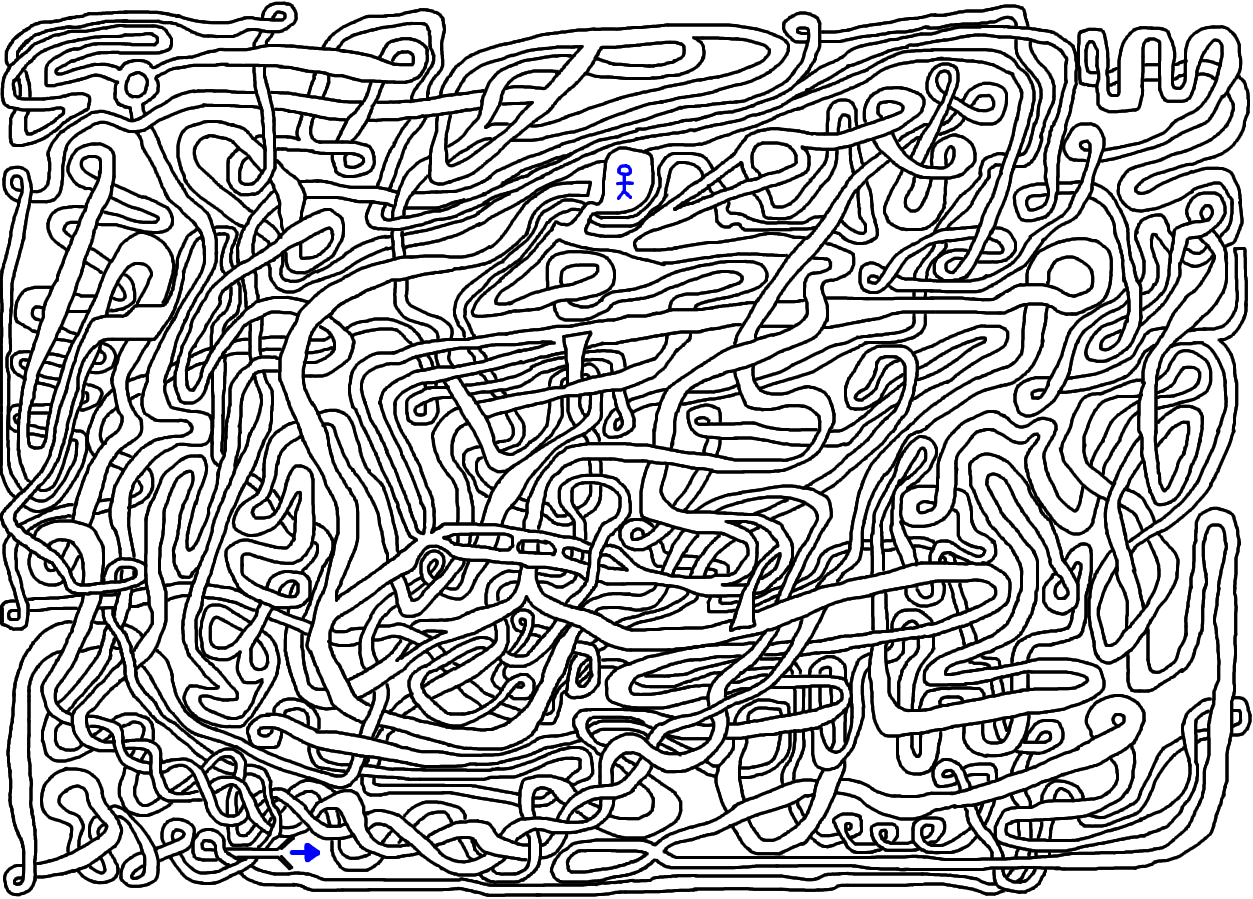
\includegraphics[width=0.4\textwidth]{img/maze.png}
\end{center}

but this computation is not performed in an automatic manner.

\end{itemise}